\documentclass[letterpaper,12pt]{article}

\usepackage{threeparttable}
\usepackage{geometry}
\geometry{letterpaper,tmargin=1in,bmargin=1in,lmargin=1.25in,rmargin=1.25in}
\usepackage[format=hang,font=normalsize,labelfont=bf]{caption}
\usepackage{amsmath}
\usepackage{multirow}
\usepackage{array}
\usepackage{delarray}
\usepackage{amssymb}
\usepackage{amsthm}
\usepackage{lscape}
\usepackage{natbib}
\usepackage{setspace}
\usepackage{float,color}
\usepackage[pdftex]{graphicx}
\usepackage{pdfsync}
\usepackage{verbatim}
\synctex=1
\usepackage{hyperref}
\hypersetup{colorlinks,linkcolor=red,urlcolor=blue,citecolor=red}
\usepackage{bm}
\theoremstyle{definition}
\newtheorem{theorem}{Theorem}
\newtheorem{acknowledgement}[theorem]{Acknowledgement}
\newtheorem{algorithm}[theorem]{Algorithm}
\newtheorem{axiom}[theorem]{Axiom}
\newtheorem{case}[theorem]{Case}
\newtheorem{claim}[theorem]{Claim}
\newtheorem{conclusion}[theorem]{Conclusion}
\newtheorem{condition}[theorem]{Condition}
\newtheorem{conjecture}[theorem]{Conjecture}
\newtheorem{corollary}[theorem]{Corollary}
\newtheorem{criterion}[theorem]{Criterion}
\newtheorem{definition}{Definition} % Number definitions on their own
\newtheorem{derivation}{Derivation} % Number derivations on their own
\newtheorem{example}[theorem]{Example}
\newtheorem{exercise}[theorem]{Exercise}
\newtheorem{lemma}[theorem]{Lemma}
\newtheorem{notation}[theorem]{Notation}
\newtheorem{problem}[theorem]{Problem}
\newtheorem{proposition}{Proposition} % Number propositions on their own
\newtheorem{remark}[theorem]{Remark}
\newtheorem{solution}[theorem]{Solution}
\newtheorem{summary}[theorem]{Summary}
\bibliographystyle{aer}
\newcommand\ve{\varepsilon}
\renewcommand\theenumi{\roman{enumi}}
\providecommand{\norm}[1]{\lVert#1\rVert}

\begin{document}

\begin{titlepage}
\title{A Macroeconomic Model for \\
       Dynamic Scoring of Tax Policy
       \thanks{
       Put thanks here.}
       }
\author{
  Jason DeBacker\footnote{Middle Tennessee State University, Department of Economics and Finance, BAS N306, Murfreesboro, TN 37132, (615) 898-2528,\href{mailto:jason.debacker@mtsu.edu}{jason.debacker@mtsu.edu}.} \\[-2pt]
  \and
  Richard W. Evans\footnote{Brigham Young University, Department of Economics, 167 FOB, Provo, Utah 84602, (801) 422-8303, \href{mailto:revans@byu.edu}{revans@byu.edu}.} \\[-2pt]
  \and
  Evan Magnusson\footnote{Brigham Young University, Department of Economics, 163 FOB, Provo, Utah 84602, \href{mailto:evanmag42@gmail.com}{evanmag42@gmail.com}.} \\[-2pt]
  \and
  Kerk L. Phillips\footnote{Brigham Young University, Department of Economics, 166 FOB, Provo, Utah 84602, (801) 422-5928, \href{mailto:kerk_phillips@byu.edu}{kerk\_phillips@byu.edu}.} \\[-2pt]
  \and
  Isaac Swift\footnote{Brigham Young University, Department of Economics, 163 FOB, Provo, Utah 84602, \href{mailto:isaacdswift@gmail.com}{isaacdswift@gmail.com}.} \\[-2pt]}
\date{August 2014 \\
  \scriptsize{(version 14.08.a)}}
\maketitle
\begin{abstract}
\normalsize{Put abstract here.

\vspace{3mm}

\noindent\textit{keywords:}\: Put keywords here.

\vspace{3mm}

\noindent\textit{JEL classification:} Put JEL codes here.}
\end{abstract}
\thispagestyle{empty}
\end{titlepage}


\begin{spacing}{1.5}

\section{Introduction}\label{SecIntro}

  Put introduction here.


\section{Model with Endogenous Labor}\label{SecModel}

  This is the basic OLG model in which households live $S$ periods and are one of $J$ ability types. The ability process is calibrated to match the wage distribution by age in the United States, and labor is endogenously supplied by individuals. The production side of the economy is characterized by a unit measure of identical, perfectly competitive firms.


  \subsection{Individual problem}\label{SecIndProb}

    A measure $\omega_{1,t}$ of individuals with heterogeneous working ability $e \in\mathcal{E}\subset\mathbb{R}_{++}$ is born in each period $t$ and live for $S\geq 3$ periods. The population of age-$s$ individuals in any period $t$ is $\omega_{s,t}$. Their working ability evolves over their lifetime according to an age-dependent deterministic process. At birth, an equal fraction $1/J$ of the $\omega_{s,t}$ measure of new agents are randomly assigned to each of the $J$ ability types indexed by $j=1,2,...J$. Once ability type is determined, that measure $\omega_{s,t}/(J)$ of individuals' ability evolves deterministically according to $e_j(s)$. The process for the evolution of the population weights $\omega_{s,t}$ is an exogenous input to the model. We calibrate the matrix of lifetime ability paths $e_j(s)$ for all types $j$ using CPS hourly wage by age distribution data.\footnote{Appendix \ref{AppAbilCalib} gives a detailed description of the calibration of the deterministic ability process by age $s$ and type $j$, as well as alternative specifications and calibrations.}

    Individuals are endowed with a measure of time $\tilde{l}$ in each period $t$, and they choose each period how much of that time to allocate between labor $n_{j,s,t}$ and leisure $l_{j,s,t}$.
    \begin{equation}\label{EqLabConstr}
      n_{j,s,t} + l_{j,s,t} = \tilde{l}
    \end{equation}

    \noindent At time $t$, all generation $s$ agents with ability $e_j(s)$ know the real wage rate $w_t$ and know the one-period real net interest rate $r_t$ on bond holdings $b_{j,s,t}$ that mature at the beginning of period $t$. In each period $t$, age-$s$ agents with working ability $e$ choose how much to consume $c_{j,s,t}$, how much to save for the next period by loaning capital to firms in the form of a one-period bond $b_{j,s+1,t+1}$, and how much to work $n_{j,s,t}$ in order to maximize expected lifetime utility of the following form,
    \begin{equation}\label{EqUtilMax}
      \begin{split}
        &U_{j,s,t} = \sum_{v=0}^{S-s}\beta^u u\left(c_{j,s+u,t+u},n_{j,s+u,t+u}\right) \\
        &\text{where} \quad u\left(c_{j,s,t},n_{j,s,t}\right) = \frac{\left(c_{j,s,t}\right)^{1-\sigma} - 1}{1-\sigma} + \chi\frac{(\tilde{l}-n_{j,s,t})^{1-\eta}}{1-\eta} \quad\forall j,s,t
      \end{split}
    \end{equation}
    where $\sigma\geq 1$ is the coefficient of relative risk aversion on consumption, $\eta\geq 1$ is proportional to the Frisch elasticity of labor supply, and $\beta\in(0,1)$ is the agent's discount factor.

    Because agents are born without any bonds maturing and because they purchase no bonds in the last period of life $s=S$, the per-period budget constraints for each agent normalized by the price of consumption are the following.
    \begin{align}
      w_t e_j(s)n_{j,s,t} &\geq c_{j,s,t} + b_{j,s+1,t+1} \quad \text{for} \quad s = 1 \quad\quad\quad\quad\:\:\: \forall j,t \label{EqBC1} \\
      \left(1 + r_t\right) b_{j,s,t} + w_t e_j(s)n_{j,s,t} &\geq c_{j,s,t} + b_{j,s+1,t+1} \quad \text{for} \quad 2\leq s \leq S-1 \quad \forall j,t \label{EqBC2} \\
      \left(1 + r_t\right) b_{j,s,t} + w_t e_j(s)n_{j,s,t} &\geq c_{j,s,t} \quad\quad\quad\quad\quad\quad \text{for} \quad s = S \quad\quad\quad\quad\:\:\, \forall j,t \label{EqBC3}
    \end{align}
    Note that the price of consumption is normalized to one, so $w_t$ is the real wage and $r_t$ is the real net interest rate.

    In addition to the budget constraints in each period, the utility function imposes nonnegative consumption through inifinite marginal utility and individual labor and leisure must be nonnegative $n_{j,s,t},l_{j,s,t}\geq 0$. We allow the possibility for individual agents to borrow $b_{j,s,t}<0$ for some $j$ and $s$ in period $t$. However, the borrowing must satisfy a series of individual feasibility constraints as well as a strict constraint that the aggregate capital stock $K_t>0$ be positive in every period.\footnote{We describe these constraints in detail in Appendix \ref{AppBorConstr}.}

    We next describe the Euler equations that govern the choices of consumption $c_{j,s,t}$ and savings $b_{j,s+1,t+1}$ by household of age $s$ and ability $e_j(s)$ in each period $t$. We work backward from the last period of life $s = S$. Because households do not save in the last period of life $b_{j,s+1,t+1}=0$ due to our assumption of no bequest motive, the household's final-period maximization problem is given by the following.
    \begin{equation}\label{EqSmaxprob}
      \begin{split}
        \max_{c_{j,S,t},n_{j,S,t},b_{j,s+1,t+1}} &\frac{\left(c_{j,S,t}\right)^{1-\sigma} - 1}{1 - \sigma} + \chi\frac{(\tilde{l}-n_{j,s,t})^{1-\eta}}{1-\eta} \\
        &\text{s.t.} \quad \left(1+r_t\right)b_{j,S,t} + w_t e_j(S)n_{j,S,t} \geq c_{j,S,t} \quad \forall t
      \end{split}
    \end{equation}
    Because $u(c)$ is monotonically increasing in $c$, the $s=S$ consumption part of the maximization problem \eqref{EqSmaxprob} is simply to choose the maximum amount of consumption possible. The household trivially consumes all of its income in the last period of life. However, the household must choose labor to balance its benefits in extra consumption with its costs in disutility.
    \begin{gather}
      c_{j,S,t} = \left(1+r_t\right)b_{j,S,t} + w_t e_j(S)n_{j,S,t} \quad \forall t \label{EqScons} \\
      w_t e_j(S)\Bigl[\left(1+r_t\right)b_{j,S,t} + w_t e_j(S)n_{j,S,t}\Bigr]^{-\sigma} = \chi(\tilde{l} - n_{j,S,t})^{-\eta} \quad\forall t \label{EqEulerSlab}
    \end{gather}

    An individual in his second-to-last period of life $s=S-1$ must choose how much to consume and how much to save for the last period of life $b_{j,S,t+1}$ as well as how much to work in the current period $n_{j,S-1,t}$ and how much to work in the final period $n_{j,S,t+1}$. The $S-1$ individual optimization problem is governed by two static first order conditions for labor  $n_{j,S-1,t}$ and $n_{j,S,t+1}$ and an intertemporal Euler equation for the savings decision.
    \begin{gather}
      \begin{split}
        w_t e_j(S-1)\Bigl[\left(1+r_t\right)b_{j,S_1,t} + w_t e_j(S-1)n_{j,S-1,t} - &b_{j,S,t+1}\Bigr]^{-\sigma} = ... \\
        &\chi(\tilde{l} - n_{j,S-1,t})^{-\eta} \quad\forall t
      \end{split} \label{EqEulerSm1lab} \\
      w_{t+1} e_j(S)\Bigl[\left(1+r_{t+1}\right)b_{j,S,t+1} + w_{t+1} e_j(S)n_{j,S,t+1}\Bigr]^{-\sigma} = \chi(\tilde{l} - n_{j,S,t+1})^{-\eta} \quad\forall t \label{EqEulerSlab2} \\
      \begin{split}
        \Bigl[\left(1+r_t\right)b_{j,S_1,t} + w_t &e_j(S-1)n_{j,S-1,t} - b_{j,S,t+1}\Bigr]^{-\sigma} = ... \\
        &\beta(1+r_{t+1})\Bigl[\left(1+r_{t+1}\right)b_{j,S,t+1} + w_{t+1} e_j(S)n_{j,S,t+1}\Bigr]^{-\sigma} \quad\forall t
      \end{split} \label{EqEulerSm1Sav}
    \end{gather}

    In general, maximizing \eqref{EqUtilMax} with respect to \eqref{EqBC1}, \eqref{EqBC2}, \eqref{EqBC3}, and the implied individual and aggregate borrowing constraints gives the following set of $S-1$ intertemporal Euler equations and $S$ static first order conditions characterizing lifetime savings $b_{j,s,t}$ for all $j$ and $2\leq s\leq S$ and labor supply $n_{j,s,t}$ for all $j$ and $1\leq s\leq S$.
    \begin{gather}
      \begin{split}
        w_t e_j(s)\Bigl[\left(1+r_t\right)b_{j,s,t} + &w_t e_j(s)n_{j,s,t} - b_{j,s+1,t+1}\Bigr]^{-\sigma} = \chi(\tilde{l} - n_{j,s,t})^{-\eta} \\
        &\forall j,t \quad\text{and}\quad 1\leq s\leq S \quad\text{with}\quad b_{j,1,t},b_{j,S+1,t}=0
      \end{split} \label{EqEulerLabGen} \\
      \begin{split}
        &\Bigl[\left(1+r_t\right)b_{j,s,t} + w_t e_j(s)n_{j,s,t} - b_{j,s+1,t+1}\Bigr]^{-\sigma} = ... \\
        &\quad \beta(1+r_{t+1})\Bigl[\left(1+r_{t+1}\right)b_{j,s+1,t+1} + w_{t+1} e_j(s+1)n_{j,s+1,t+1} - b_{j,s+2,t+2}\Bigr]^{-\sigma} \\
        &\quad\quad\quad\quad\quad\quad\quad\quad\forall j,t \quad\text{and}\quad 1\leq s\leq S-1 \quad\text{with}\quad b_{j,1,t},b_{j,S+1,t}=0
      \end{split} \label{EqEulerSavGen}
    \end{gather}


  \subsection{Firm problem}\label{SecModelGenFirm}

    A unit measure of identical, perfectly competitive firms exist in this economy. The representative firm is characterized by the following Cobb-Douglas production technology,
    \begin{equation}\label{EqCobbDougProd}
       Y_t = A_t K_t^\alpha L_t^{1-\alpha} \quad \forall t
    \end{equation}
    where $A_t$ is the technology process with possible growth over time and $\alpha\in(0,1)$ and $L_t$ is measured in efficiency units of labor. The interest rate $r_t$ in the cost function is a net real interest rate because depreciation $\delta$ is paid by the firms. The real wage is $w_t$. The real profit function of the firm is the following.
    \begin{equation}\label{EqFirmProfit}
       \text{Real Profits} = A_t K_t^\alpha L_t^{1-\alpha} - (r_t + \delta)K_t - w_t L_t
    \end{equation}
    As in the budget constraints \eqref{EqBC1}, \eqref{EqBC2}, and \eqref{EqBC3}, note that the price of the good has been normalized to one.

    Profit maximization results in the real wage $w_t$ and the real rental rate of capital $r_t$ being determined by the marginal products of labor and capital, respectively.
    \begin{align}
       w_t &= (1-\alpha)\frac{Y_t}{L_t} \quad \forall t \label{EqFOCwage}\\
       r_t &= \alpha\frac{Y_t}{K_t} - \delta \quad\:\:\: \forall t \label{EqFOCrate}
    \end{align}


  \subsection{Market clearing and equilibrium}\label{SecMCandEqlbm}

    Labor market clearing requires that aggregate labor demand $L_t$ measured in efficiency units equal the sum of individual efficiency labor supplied $e_j(s)n_{j,s,t}$. Capital market clearing requires that aggregate capital demand $K_t$ equal the sum of capital investment by households $b_{j,s,t}$. Aggregate consumption $C_t$ is defined as the sum of all individual consumptions, and investment is defined by the standard $Y = C + I$ constraint as shown in \eqref{EqMktClrGoods}.
    \begin{align}
      L_t &= \frac{1}{J}\sum_{s=1}^S\sum_{j=1}^{J} \omega_{s,t}e_j(s)n_{j,s,t} \quad\quad \forall t \label{EqMktClrLab} \\
      K_t &= \frac{1}{J}\sum_{s=1}^{S}\sum_{j=1}^{J}\omega_{s,t}b_{j,s,t} \quad\quad\quad\quad \forall t \label{EqMktClrCap} \\
      \begin{split}
        Y_t &= C_t + K_{t+1} - (1-\delta)K_t \quad\forall t \\
        &\quad\text{where}\quad C_t \equiv \frac{1}{J}\sum_{s=1}^{S}\sum_{j=1}^{J}\omega_{s,t}c_{j,s,t}
      \end{split} \label{EqMktClrGoods}
    \end{align}
    The steady-state equilibrium for this economy is defined as follows.

    \vspace{7mm}
    \end{spacing}
    \hrule
    \begin{definition}[\textbf{Steady-state equilibrium}]\label{DefEquilSS}
      A non-autarkic steady-state equilibrium in the overlapping generations model with $S$-period lived agents and heterogeneous ability $e_j(s)$ is defined as constant allocations $c_{j,s,t}=\bar{c}_{j,s}$, $b_{j,s+1,t+1}=\bar{b}_{j,s+1}$, and $n_{j,s,t}=\bar{n}_{j,s}$ and constant prices $w_t=\bar{w}$ and $r_t=\bar{r}$ for all $j$, $s$, and $t$ such that the following conditions hold:
       \begin{enumerate}
          \item households optimize according to \eqref{EqSmaxprob}, \eqref{EqScons}, \eqref{EqEulerLabGen}, and \eqref{EqEulerSavGen},
          \item firms optimize according to \eqref{EqFOCwage} and \eqref{EqFOCrate}, and
          \item markets clear according to \eqref{EqMktClrLab}, \eqref{EqMktClrCap}, and \eqref{EqMktClrGoods}.
       \end{enumerate}
    \end{definition}
    \hrule
    \begin{spacing}{1.5}
    \vspace{10mm}

    The steady-state equilibrium is characterized by the system of $J(2S-1)$ equations and $J(2S-1)$ unknowns $\bar{n}_{j,s}$ and $\bar{b}_{j,s+1}$ along with the individual borrowing constraints and aggregate borrowing constraint described in Appendix \ref{AppBorConstr}.

    \begin{gather}
      \begin{split}
        \bar{w}e_j(s)\Bigl[\left(1+\bar{r}\right)\bar{b}_{j,s} + &\bar{w} e_j(s)\bar{n}_{j,s} - \bar{b}_{j,s+1}\Bigr]^{-\sigma} = \chi(\tilde{l} - \bar{n}_{j,s})^{-\eta} \\
        &\forall j \quad\text{and}\quad 1\leq s\leq S \quad\text{with}\quad \bar{b}_{j,1},\bar{b}_{j,S+1}=0
      \end{split} \label{EqEulerLabGenSS} \\
      \begin{split}
        &\Bigl[\left(1+\bar{r}\right)\bar{b}_{j,s} + \bar{w}e_j(s)\bar{n}_{j,s} - \bar{b}_{j,s+1}\Bigr]^{-\sigma} = ... \\
        &\quad\quad\quad \beta(1+\bar{r})\Bigl[\left(1+\bar{r}\right)\bar{b}_{j,s+1} + \bar{w}e_j(s+1)\bar{n}_{j,s+1} - \bar{b}_{j,s+2}\Bigr]^{-\sigma} \\
        &\quad\quad\quad\quad\quad\quad\quad\quad\forall j \quad\text{and}\quad 1\leq s\leq S-1 \quad\text{with}\quad \bar{b}_{j,1},\bar{b}_{j,S+1}=0
      \end{split} \label{EqEulerSavGenSS}
    \end{gather}

    Define $\bm{\Gamma}_t$ as the distribution of savings across individuals at time $t$.
    \begin{equation}\label{EqSavDist}
      \bm{\Gamma}_t \equiv \{b_{j,s,t}\}_{j=1,s=2}^{J,S} \quad\forall t
    \end{equation}
    In equilibrium, the steady-state individual labor supplies $\bar{n}_{j,s}$ for all $j$ and $s$, the steady-state real wage $\bar{w}$, and the steady-state real rental rate $\bar{r}$ are simply functions of the steady-state distribution of savings $\bar{\Gamma}$. This is clear from the steady-state version of the capital market clearing condition \eqref{EqMktClrCap} and the fact that aggregate labor supply is a function of the sum of exogenous efficiency units of labor in the labor market clearing condition \eqref{EqMktClrLab}. And the two firm first order conditions for the real wage $w_t$ \eqref{EqFOCwage} and real rental rate $r_t$ \eqref{EqFOCrate} are only functions of the aggregate capital stock $K_t$ and aggregate labor $L_t$. Appendix \ref{AppSSsolve} details how to solve for the steady-state equilibrium.

    \begin{figure}[htb]\centering \captionsetup{width=4.0in}
      \caption{\label{FigSavSS}\textbf{Steady-state distribution of savings $\bar{\bm{\Gamma}}$ for $S=60$ and $J=7$}}
      \fbox{\resizebox{4.0in}{3.0in}{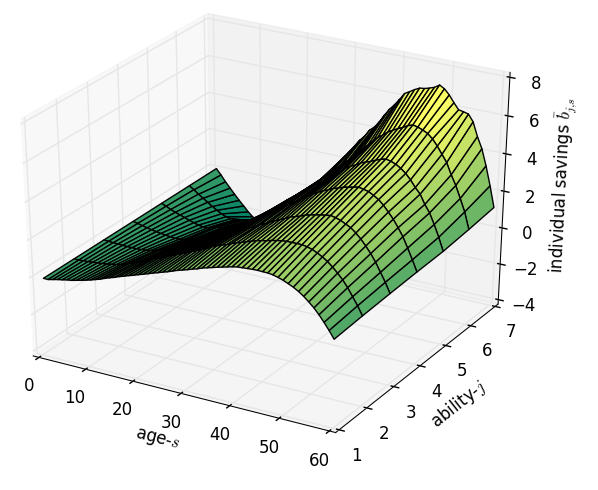
\includegraphics{images/SavSS.png}}}
    \end{figure}

    \begin{figure}[htb]\centering \captionsetup{width=4.0in}
      \caption{\label{FigLabSS}\textbf{Steady-state distribution of individual labor supply $\bar{n}_{j,s}$ for $S=60$ and $J=7$}}
      \fbox{\resizebox{4.0in}{3.0in}{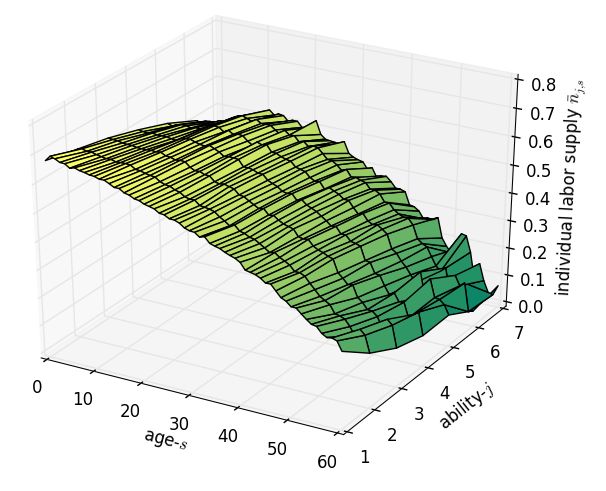
\includegraphics{images/LabSS.png}}}
    \end{figure}

    Figure \ref{FigSavSS} shows the steady-state distribution of individual savings $\bar{\bm{\Gamma}}$ and Figure \ref{FigLabSS} shows the steady-state distribution of individual labor supply $\bar{n}_{j,s}$ for a particular calibration of the model. The deterministic individual ability process $e_j(s)$ is calibrated from CPS wage distribution data as described in Appendix \ref{AppAbilCalib}, with $S=60$ and $J=7$. We calibrate the other parameters to $[\beta,\sigma,\delta,\chi,\eta,\alpha,A] = [0.96,3,0.05,1,2,0.35,1]$. Notice .... %that some intergenerational risk sharing is taking place. Young individuals of high ability, know that they will have high ability and borrow $b_{j,s,t}<0$ in their early years in the steady-state.

    The definition of the non-steady-state equilibrium is similar to Definition \ref{DefEquilSS}, with the steady-state equilibrium definition being a special case of the non-steady-state equilibrium.

    \vspace{7mm}
    \end{spacing}
    \hrule
    \begin{definition}[\textbf{Non-steady-state equilibrium}]\label{DefEquilNonSS}
      A non-autarkic non-steady-state equilibrium in the overlapping generations model with $S$-period lived agents and heterogeneous ability $e_j(s)$ is defined as allocations $c_{j,s,t}$, $n_{j,s,t}$ and $b_{j,s+1,t+1}$ and prices $w_t$ and $r_t$ for all $j$, $s$, and $t$ such that the following conditions hold:
       \begin{enumerate}
          \item households optimize according to \eqref{EqSmaxprob}, \eqref{EqScons}, \eqref{EqEulerLabGen}, and \eqref{EqEulerSavGen},
          \item firms optimize according to \eqref{EqFOCwage} and \eqref{EqFOCrate}, and
          \item markets clear according to \eqref{EqMktClrLab}, \eqref{EqMktClrCap}, and \eqref{EqMktClrGoods}.
       \end{enumerate}
    \end{definition}
    \hrule
    \begin{spacing}{1.5}
    \vspace{10mm}

    \noindent The household labor-leisure decision in the last period of life shows that the optimal labor supply for age $s=S$ is a function of individual holdings of savings and the prices in that period $n_{j,S,t}=\phi\bigl(b_{j,S,t},w_t,r_t\bigr)$. This decision is characterized by final-age Euler equation \eqref{EqEulerSlab}. Households in their second-to-last period of life in period $t$ have three decisions to make. They must choose how much to work this period $n_{j,S-1,t}$ and next $n_{j,S,t+1}$ and how much to save this period for next period $b_{j,S,t+1}$. The optimal responses for this individual are characterized by the first order conditions \eqref{EqEulerSm1lab}, \eqref{EqEulerSlab2}, and \eqref{EqEulerSm1Sav}, respectively.

    The optimal labor supply at age $s=S-1$ is a function of the current savings and the current prices $n_{j,S-1,t}=\phi\bigl(b_{j,S-1,t},w_t,r_t\bigr)$, and the optimal labor supply at age $s=S$ is a function of the next period's prices $n_{j,S,t+1}=\phi\bigl(b_{j,S,t+1},w_{t+1},r_{t+1}\bigr)$. However, optimal savings in the second-to-last period of life is a function of the current savings and the prices in the current period and in the next period $b_{j,S,t+1} = \psi\bigl(b_{j,S-1,t},w_t,r_t,w_{t+1},r_{t+1}\bigr)$. By induction, we can show that the optimal labor supply function for any individual with ability $j$, age $s$, and in period $t$ is a function of current holdings of savings and the current period prices.
    \begin{equation}\label{EqLabPolFuncGen}
      n_{j,s,t} = \phi\bigl(b_{j,s,t},w_t,r_t\bigr) \quad\forall j,s,t
    \end{equation}
    We can also show that the solution to the households saving decision in any period is a function of their current holdings of savings and the series of prices over the rest of their life.
    \begin{equation}\label{EqSavPolFuncGen}
      b_{j,s+1,t+1} = \psi\Bigl(b_{j,s,t},(w_v,r_v)_{v=t}^{t+S-s}\Bigr) \quad\forall j,t \quad\text{and}\quad 1\leq s\leq S-1
    \end{equation}

    Each optimal saving decision for each household requires knowledge of at least todays prices and tomorrows prices and at most $S$ periods of prices. In equilibrium, one can see that the prices $(w_t,r_t)$ in each period $t$ are functions of the entire distribution of savings $\bm{\Gamma}_t$. The requirement that individuals be able to forecast prices with perfect foresight over their lifetimes implies that each individual has correct information and beliefs about all the other individuals optimization problems and information. It also implies that the equilibrium allocations and prices are really just functions of the entire distribution of savings at a particular period, as well as a law of motion for that distribution of savings.

    \begin{figure}[htb]\centering \captionsetup{width=4.0in}
      \caption{\label{FigKpathTPI}\textbf{Equilibrium time path of $K_t$ for $S=60$ and $J=7$}}
      \fbox{\resizebox{4.0in}{3.0in}{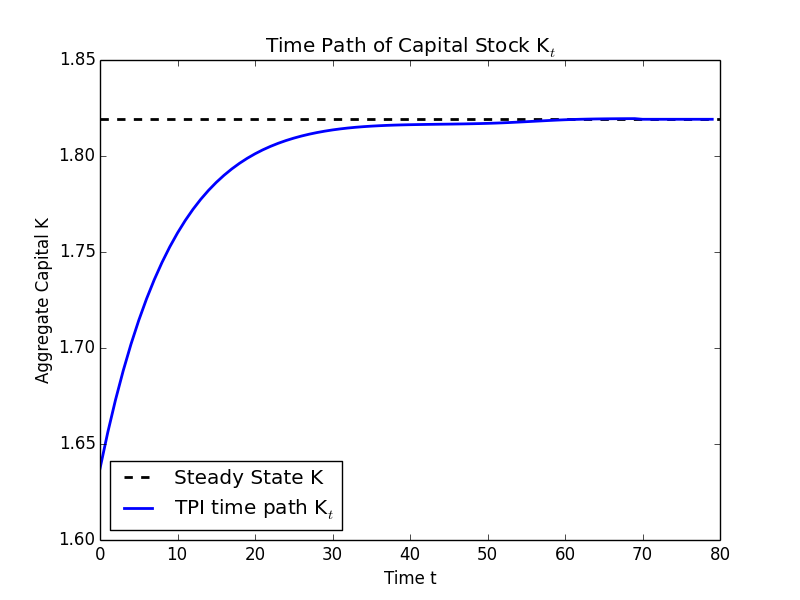
\includegraphics{images/KpathTPI.png}}}
    \end{figure}

    To solve for any non-steady-state equilibrium time path of the economy from an arbitrary current state to the steady state, we follow the time path iteration (TPI) method of \citet{AuerbachKotlikoff:1987}. Appendix \ref{AppNonSSsolve} details how to solve for the non-steady-state equilibrium time path using the TPI method. Figure \ref{FigKpathTPI} shows the equilibrium time path of the aggregate capital stock for the calibration used in Figure \ref{FigKpathTPI} for $T=80$ periods starting from an initial distribution of savings in which $b_{j,s,1}=(0.9\bar{K})/[(S-1)J]$ for all $j$ and $s$. We used $\rho=0.2$ as our time-path updating parameter (see Equation \eqref{EqTPInewpath} in Appendix \ref{AppNonSSsolve}.)


\clearpage

\end{spacing}

\newpage
\renewcommand{\theequation}{A.\arabic{section}.\arabic{equation}}
                                                 % redefine the command that creates the section number
\renewcommand{\thesection}{A-\arabic{section}}   % redefine the command that creates the equation number
\setcounter{equation}{0}                         % reset counter
\setcounter{section}{0}                          % reset section number
\section*{APPENDIX}                              % use *-form to suppress numbering

\section{Calibration of ability process}\label{AppAbilCalib}

  The calibration of the ability process $e_j(s)$ is as follows.  First, the ability types themselves must be calibrated. For each age group $s \in S$, the hourly wage rates are sorted into $J$ percentile groups.  The ability type for each percentile group is the median wage for the percentile group, divided by the average wage of all individuals in the data set.

  The data used to calibrate the ability types were obtained from the Current Population Survey.\footnote{U.S. Census Bureau, Dataferret, Current Population Survey, 2014. The variables $PRTAGE$, $PTERNHLY$, and $PWCMPWGT$ were used for the age, hourly wage rate, and population weight of individuals, respectively. \\ [-2pt]} Individuals younger than 20 and older than 79 are dropped from the data. This is due to the extremely small amount of observations for ages outside of those bounds. Due to a limited number of observations in the survey who included their hourly wage, data was taken from the months of January, February, March, April, and May 2014.  Population weights were also used to obtain the correct percentile groups of individuals.  The income levels for the $J$ ability types were then calculated for each month, and then an average was taken of the five calibrations of the ability types in order to produce a final calibration to be used in the model. Figure \ref{FigIncome} shows this income distribution across age and ability type.

    \begin{figure}[htb]\centering \captionsetup{width=4.0in}
      \caption{\label{FigIncome}\textbf{Distribution of Income where $S=60$ and $J=7$}}
      \fbox{\resizebox{4.0in}{2.8in}{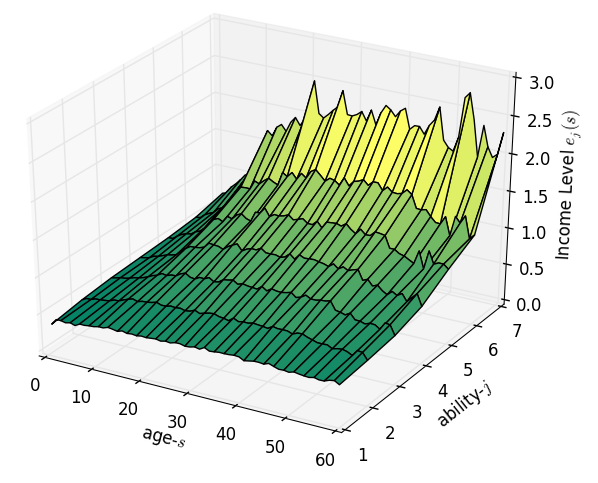
\includegraphics{images/income.png}}}
    \end{figure}

  In this paper, individuals are assigned ability types at the beginning of their life, and cannot change types later on.
% Do we need to cite the data set sources? (for both e and f)


\newpage
\section{Constraints on individual borrowing}\label{AppBorConstr}

  \setcounter{equation}{0}

  As described in Section \ref{SecIndProb}, individuals are allowed to borrow $b_{j,s,t}$ for some $j$ and $s$ in period $t$. However, two constraints must hold. First, the individual must be able to pay back the balance with interest $r_{t+1}$ in the next period without driving consumption in the next period $c_{j,s+1,t+1}$ to be nonpositive. Let $\tilde{b}_{j,s,t}$ be the minimum value of savings in a period.
  \begin{equation}\label{EqSavMin}
    b_{j,s,t}\geq\tilde{b}_{j,s,t} \quad\forall j,s,t
  \end{equation}
  Rearranging the bugdet constraints in \eqref{EqBC1}, \eqref{EqBC2}, and \eqref{EqBC3} and using backward induction gives the following expressions for $\bar{b}_{j,s,t}$,
  \begin{equation}\label{EqBorConsts}
    \begin{split}
      \tilde{b}_{j,S,t} &= \frac{\tilde{c} - w_te_j(S)\tilde{l}}{1+r_t}  \\
      \tilde{b}_{j,S-1,t-1} &= \frac{\tilde{c} + \tilde{b}_{j,S,t} - w_{t-1}e_j(S-1)\tilde{l}}{1+r_{t-1}} \\
      &\vdots \\
      \tilde{b}_{j,2,t-S+2} &= \frac{\tilde{c} + \tilde{b}_{j,3,t-S+3} - w_{t-S+2}e_j(2)\tilde{l}}{1+r_{t-S+2}}
    \end{split}
  \end{equation}
  where $\tilde{c}>0$ is some minimum amount of consumption and $\tilde{l}$ is the maximum amount an individual can work from the time constraint \eqref{EqLabConstr}. With endogenous labor supply $n_{j,s,t}$, it is less likely that the individual borrowing constraints every bind. This is because the disutility of labor increases exponentially according to $\eta>1$ in the period utility function \eqref{EqUtilMax}.

  In addition to the individual borrowing constraint \eqref{EqSavMin}, a strict aggregate borrowing constraint must be met. That is, the aggregate capital stock must be strictly positive.
  \begin{equation}\label{EqAggrCapConstr}
    K_t > 0 \quad\forall t
  \end{equation}


\newpage
\section{Solving for steady-state equilibrium}\label{AppSSsolve}

  \setcounter{equation}{0}
  \renewcommand\theenumi{\arabic{enumi}}
  \renewcommand\theenumii{\alph{enumii}}
  \renewcommand\theenumiii{\roman{enumiii}}

  This section describes the solution method for the steady-state equilibrium described in Definition \ref{DefEquilSS}.

  \begin{enumerate}
    \item Choose an initial guess for the steady-state distribution of capital $\bar{b}_{j,s+1}$ for all $j$ and $s=1,2,...S-1$ and labor supply $\bar{n}_{j,s}$ for all $j$ and $s$.
      \begin{itemize}
        \item A good first guess is a large positive number for all the $\bar{n}_{j,s}$ that is slightly less than $\tilde{l}$ and to choose some small positive number that is small enough to be less than the minimum income that an individual might have $\bar{w}e_j(s)\bar{n}_{j,s}$.
      \end{itemize}
    \item Perform an unconstrained root finder that chooses $\bar{b}_{j,s+1}$ that solves the $J\times(S-1)$ steady-state Euler equations \eqref{EqSSeuler}.
    \item Make sure none of the implied steady-state consumptions $\bar{c}_{j,s,t}$ is less-than-or-equal-to zero.
      \begin{itemize}
        \item If one consumption is less-than-or-equal-to zero $\bar{c}_{j,s}\leq 0$, then try different starting values.
        \item If that does not work, then we must perform the root finding operation as a constrained minimization problem that puts a maximum value on $\bar{b}_{j,s+1}$.
      \end{itemize}
    \item Make sure that none of the Euler errors is too large in absolute value. A steady-state Euler error is the following, which is supposed to be close to zero for all $j$ and $s=1,2,...S-1$:
      \begin{equation}\label{EqSSeulerr}
        \frac{\beta \left(1+\bar{r}\right)\left(\bar{c}_{j,s+1}\right)^{-\sigma}}{\left(\bar{c}_{j,s}\right)^{-\sigma}} - 1
      \end{equation}
    \item Make sure that the unconstrained solution satisfies the individual borrowing constraints in \eqref{EqSavMin} and \eqref{EqBorConsts}.
      \begin{itemize}
        \item If any individual's borrowing constraint is not satisfied using the unconstrained root finding operation, rerun the root finding operation in step (ii) as a constrained minimization problem with the borrowing constraints imposed on those individuals.
        \item Repeat steps (ii) through (v) until all the individual borrowing constraints are met.
      \end{itemize}
    \item Make sure that the solution satisfies the aggregate borrowing constraint \eqref{EqAggrCapConstr}.
      \begin{itemize}
        \item If it does not, what is the least distortionary upward adjustment to individual steady-state savings $\bar{b}_{j,s+1}$?
      \end{itemize}
  \end{enumerate}


\newpage
\section{Solving for non-steady-state equilibrium by time path iteration}\label{AppNonSSsolve}

  \setcounter{equation}{0}

  This section outlines the benchmark time path iteration (TPI) method of \citet{AuerbachKotlikoff:1987} for solving the non-steady-state equilibrium transition path of the distribution of savings. TPI finds a fixed point for the transition path of the distribution of capital for a given initial state of the distribution of capital. The idea is that the economy is infinitely lived, even though the agents that make up the economy are not. Rather than recursively solving for equilibrium policy functions by iterating on individual value functions, one must recursively solve for the policy functions by iterating on the entire transition path of the endogenous objects in the economy (see \citet[ch. 17]{StokeyLucas:1989}).

  The key assumption is that the economy will reach the steady-state equilibrium described in Definition \ref{DefEquilSS} in a finite number of periods $T<\infty$ regardless of the initial state. Let $\bm{\Gamma}_t$ represent the distribution of savings at time $t$.
  \begin{equation}\tag{\ref{EqSavDist}}
    \bm{\Gamma}_t \equiv \{b_{j,s,t}\}_{j=1,s=1}^{J,S} \quad\forall t
  \end{equation}
  In Section \ref{SecMCandEqlbm}, we described how the equilibrium non-steady-state time path of allocations and price is described by functions of the state $\bm{\Gamma}_t$ and its law of motion. TPI starts the economy at any initial distribution of savings $\bm{\Gamma}_0$ and solves for its equilibrium time path over $T$ periods to the steady-state distribution $\bar{\bm{\Gamma}}_T$.

  The first step is to assume an initial transition path for aggregate capital $\mathbf{K}^i = \left\{K_1^i,K_2^i,...K_T^i\right\}$ such that $T$ is sufficiently large to ensure that $\bm{\Gamma}_T = \bar{\bm{\Gamma}}$ and $K_T^i\left(\bm{\Gamma}_T\right) = \bar{K}\left(\bar{\bm{\Gamma}}\right)$. The superscript $i$ is an index for the iteration number. The transition path for aggregate capital determines the transition path for both the real wage $\bm{w}^i = \left\{w_1^i,w_2^i,...w_T^i\right\}$ and the real return on investment $\bm{r}^i = \left\{r_1^i,r_2^i,...r_T^i\right\}$. The exact initial distribution of capital in the first period $\bm{\Gamma}_1$ can be arbitrarily chosen as long as it satisfies $K_1^i = \frac{1}{SJ}\sum_{s=1}^{S}\sum_{j=1}^{J}b_{j,s,t}$ according to market clearing condition \eqref{EqMktClrCap}. One could also first choose the initial distribution of savings $\bm{\Gamma}_1$ and then choose an initial aggregate capital stock $K_1^i$ that corresponds to that distribution. As mentioned earlier, the only other restriction on the initial transition path for aggregate capital is that it equal the steady-state level $K_T^i = \bar{K}\left(\bar{\bm{\Gamma}}\right)$ by period $T$. \citet{EvansPhillips:2014} have shown that the aggregate capital stocks $K_t^i$ for periods $1<t<T$ can take on almost any positive values.

  Given the initial capital distribution $\bm{\Gamma}_1$ and the transition paths of aggregate capital $\bm{K}^i = \left\{K_1^i,K_2^i,...K_T^i\right\}$, the real wage $\bm{w}^i = \left\{w_1^i,w_2^i,...w_T^i\right\}$, and the real return to investment $\bm{r}^i = \left\{r_1^i,r_2^i,...r_T^i\right\}$, one can solve for the optimal savings policy rule for each type $j$ of $S-1$-aged agent for the last period of his life $b_{j,S,2} = \psi_{j,S-1}(b_{j,S-1,1},\{w_t,r_t\}_{t=1}^2)$ using his one intertemporal Euler equation \eqref{EqEulerSm1p1}, where the ``j,S-1" subscript on $\psi$ represents the function for type $j$ in age $s=S-1$ savings decision.
  \begin{equation}\label{EqEulerSm1p1}
    \begin{split}
      &\Bigl([1+r_1^i]b_{j,S-1,1} + w_1^i e_j(S-1)l(S-1) - b_{j,S,2}\Bigr)^{-\sigma} = \\
      &\quad\quad\quad\quad\quad\quad\quad \beta(1+r_2^i)\Bigl([1+r_2^i]b_{j,S,2} + w_2^i e_j(S)l(S)\Bigr)^{-\sigma} \quad\forall j
    \end{split}
  \end{equation}

  The final two savings decisions of each type $j$ of $S-2$-aged household in period 1, $b_{j,S-1,2}$ and $b_{j,S,3}$, are characterized by the following two intertemporal Euler equations.
  \begin{equation}\label{EqEulerSm2p1}
    \begin{split}
      &\Bigl([1+r_1^i]b_{j,S-2,1} + w_1^i e_j(S-2)l(S-2) - b_{j,S-1,2}\Bigr)^{-\sigma} = \\
      &\quad\quad\quad\quad \beta(1+r_2^i)\Bigl([1+r_2^i]b_{j,S-1,2} + w_2^i e_j(S-1)l(S-1) - b_{j,S,3}\Bigr)^{-\sigma}, \\
      &\Bigl([1+r_2^i]b_{j,S-1,2} + w_2^i e_j(S-1)l(S-1) - b_{j,S,3}\Bigr)^{-\sigma} = \\
      &\quad\quad\quad\quad\quad\quad \beta(1+r_3^i)\Bigl([1+r_3^i]b_{j,S,3} + w_3^i e_j(S)l(S)\Bigr)^{-\sigma}
    \end{split} \quad\forall j
  \end{equation}

  This process is repeated for every age of household alive in $t=1$ down to the age $s=1$ household at time $t=1$. Each of these households $j$ solve the full set of $S-1$ savings decisions characterized by the following equations.
  \begin{equation}\label{EqEulerFullp1}
    \begin{split}
      &\Bigl(w_1^i e_j(1)l(1) - b_{j,2,2}\Bigr)^{-\sigma} = ... \\
      &\quad\quad\quad\quad\quad \beta\left(1+r_2^i\right)\Bigl(\bigl[1+r_2^i\bigr]b_{j,2,2} + w_2^i e_j(2)l(2) - b_{j,3,3}\Bigr)^{-\sigma} \\
      &\Bigl(\bigl[1+r_2^i\bigr]b_{j,2,2} + w_2^i e_j(2)l(2) - b_{j,3,3}\Bigr)^{-\sigma} = ... \\
      &\quad\quad\quad\quad\quad \beta\left(1 + r_3^i\right)\Bigl(\bigl[1+r_3^i\bigr]b_{j,3,3} + w_3^i e_j(3)l(3) - b_{j,4,4}\Bigr)^{-\sigma} \\
      &\quad\quad\quad\quad\quad\quad\quad\quad\vdots \\
      &\Bigl(\bigl[1 + r_{S-1}^i\bigr]b_{j,S-1,S-1} + w_{S-1}^i e_j(S-1)l(S-1) - b_{S,S}\Bigr)^{-\sigma} = ... \\
      &\quad\quad\quad\quad\quad \beta\left(1 + r_S^i\right)\Bigl(\bigl[1+r_S^i\bigr]b_{j,S,S} + w_S^i e_j(S)l(S)\Bigr)^{-\sigma}
    \end{split}\quad\forall j
  \end{equation}

  We can then solve for the entire lifetime of savings decisions for each age $s=1$ individual in periods $t=2,3,...T$. The central part of the schematic diagram in Figure \ref{FigTPIdiag} shows how this process is done in order to solve for the equilibrium time path of the economy from period $t=1$ to $T$. Note that for each full lifetime savings path solved for an individual born in period $t\geq 2$, we can solve for the aggregate capital stock implied by those savings decisions $K_t^{i'}=\frac{1}{SJ}\sum_{s=1}^S\sum_{j=1}^J b_{j,s,t}$.

  \begin{figure}[htb]\centering \captionsetup{width=4.0in}
    \caption{\label{FigTPIdiag}\textbf{Diagram of TPI solution method within each iteration for $S=4$ and $J=1$}}
    \fbox{\resizebox{4.0in}{5.0in}{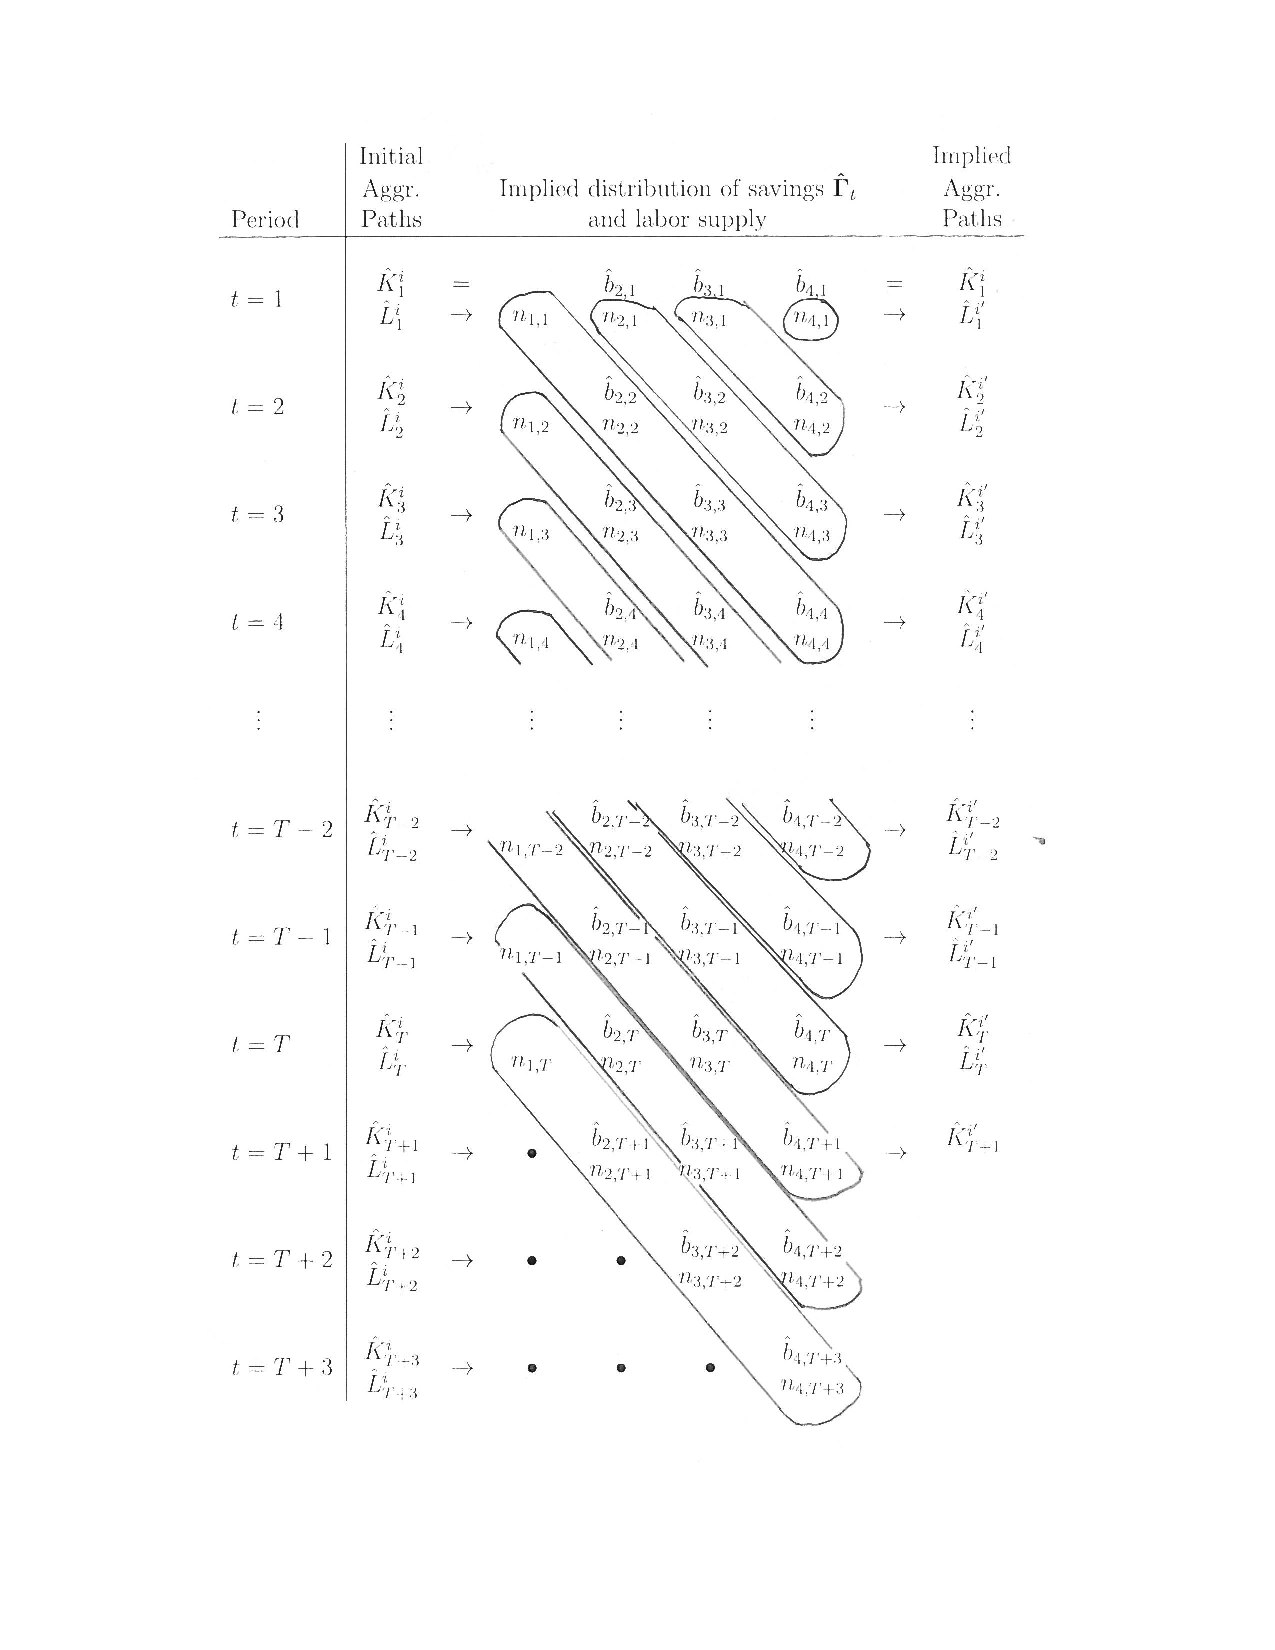
\includegraphics{images/TPIdiag.pdf}}}
  \end{figure}

  % THIS IS THE CODE FOR THE TABLE UNDERLYING THE FIGURE ABOVE
  % \begin{tabular}{>{\normalsize}l| >{\normalsize}c >{\normalsize}c >{\normalsize}c >{\normalsize}c >{\normalsize}c >{\normalsize}c >{\normalsize}c}
  %          & Initial & & & & & & Implied \\
  %          & Capital & & \multicolumn{3}{c}{Implied distribution} & & Capital \\
  %   Period & Path    & & \multicolumn{3}{c}{of savings $\bm{\Gamma}_t$}   & & Path    \\
  %   \hline
  %   & & & & & & & \\
  %   $t=1$ & $K_1^i$ & $=$ & $b_{2,1}$ & $b_{3,1}$ & $b_{4,1}$ & $=$ & $K_1^i$ \\[8mm]
  %   $t=2$ & $K_2^i$ & $\rightarrow$ & $b_{2,2}$ & $b_{3,2}$ & $b_{4,2}$ & $\rightarrow$ & $K_2^{i'}$ \\[8mm]
  %   $t=3$ & $K_3^i$ & $\rightarrow$ & $b_{2,3}$ & $b_{3,3}$ & $b_{4,3}$ & $\rightarrow$ & $K_3^{i'}$ \\[8mm]
  %   $t=4$ & $K_4^i$ & $\rightarrow$ & $b_{2,4}$ & $b_{3,4}$ & $b_{4,4}$ & $\rightarrow$ & $K_4^{i'}$ \\[8mm]
  %   $\quad\vdots$ & $\vdots$ & & $\vdots$ & $\vdots$ & $\vdots$ & & $\vdots$ \\[8mm]
  %   $t=T-2$ & $K_{T-2}^i$ & $\rightarrow$ & $b_{2,T-2}$ & $b_{3,T-2}$ & $b_{4,T-2}$ & $\rightarrow$ & $K_{T-2}^{i'}$ \\[8mm]
  %   $t=T-1$ & $K_{T-1}^i$ & $\rightarrow$ & $b_{2,T-1}$ & $b_{3,T-1}$ & $b_{4,T-1}$ & $\rightarrow$ & $K_{T-1}^{i'}$ \\[8mm]
  %   $t=T$ & $K_{T}^i$ & $\rightarrow$ & $b_{2,T}$ & $b_{3,T}$ & $b_{4,T}$ & $\rightarrow$ & $K_T^{i'}$ \\[8mm]
  %   $t=T+1$ & $K_{T+1}^i$ & $\rightarrow$ & $\bullet$ & $b_{3,T+1}$ & $b_{4,T+1}$ & $\rightarrow$ & $K_{T+1}^{i'}$ \\[8mm]
  %   $t=T+2$ & $K_{T+2}^i$ & $\rightarrow$ & $\bullet$ & $\bullet$ & $b_{4,T+2}$ & $\rightarrow$ & $K_{T+2}^{i'}$ \\
  % \end{tabular}

  Once the set of lifetime saving decisions has been computed for all individuals alive in $1\leq t\leq T$, we use the household decisions to compute a new implied time path of the aggregate capital stock. The implied path of the aggregate capital stock $\bm{K}^{i'}=\{K_1^i,K_2^{i'},...K_T^{i'}\}$ in general does not equal the initial path of the aggregate capital stock $\bm{K}^{i}=\{K_1^i,K_2^{i},...K_T^{i}\}$ that was used to compute the household savings decisions $\bm{K}^{i'}\neq\bm{K}^i$.

  Let $\norm{\:\cdot\:}$ be a norm on the space of time paths of the aggregate capital stock $\bm{K}\in\mathcal{K}\subset\mathbb{R}_{++}^T$. Then the fixed point necessary for the equilibrium transition path from Definition \ref{DefEquilNonSS} has been found when the distance between $\bm{K}^{i'}$ and $\bm{K}^{i}$ is arbitrarily close to zero.
  \begin{equation}\label{EqTPIconverge}
    \norm{\bm{K}^{i'} - \bm{K}^{i}} \leq \ve \quad\text{for}\quad \ve>0
  \end{equation}
  If the fixed point has not been found $\norm{\bm{K}^{i'} - \bm{K}^{i}} > \ve$, then a new transition path for the aggregate capital stock is generated as a convex combination of $\bm{K}^{i'}$ and $\bm{K}^{i}$.
  \begin{equation}\label{EqTPInewpath}
    \bm{K}^{i+1} = \rho\bm{K}^{i'} + (1-\rho)\bm{K}^{i} \quad\text{for}\quad \rho\in(0,1)
  \end{equation}
  This process is repeated until the initial transition path for the aggregate capital stock is consistent with the transition path implied by those beliefs and household and firm optimization.

  In essence, the TPI method iterates on individual beliefs about the time path of prices represented by a time path for the aggregate capital stock $\bm{K}^i$ until a fixed point in beliefs is found that are consistent with the transition path implied by optimization based on those beliefs.

  The following are the steps for computing a non-steady-state equilibrium time path for the economy.
  \begin{enumerate}
    \item Using the parameterization from the steady-state computation, and choose the value for $T$ at which the non-steady-state transition path should have converged to the steady state.
    \item Choose an initial state of the aggregate capital stock $K_1$. Choose an initial distribution of savings $\bm{\Gamma}_1$ consistent with $K_1$ according to \eqref{EqMktClrCap}.
    \item Conjecture a transition path for the aggregate capital stock $\bm{K}^i=\{K^i_t\}_{t=1}^\infty$ where the only requirements are that $K^i_1=K_1$ is your initial state and that $K^i_t=\bar{K}$ for all $t\geq T$. The conjectured transition path of the aggregate capital stock $\bm{K}^i$, along with the exogenous aggregate labor supply from \eqref{EqMktClrLab}, implies specific transition paths for the real wage $\bm{w}^i=\{w^i_t\}_{t=1}^\infty$ and the real interest rate $\bm{r}^i=\{r^i_t\}_{t=1}^\infty$ through expressions \eqref{EqCobbDougProd}, \eqref{EqFOCwage}, and \eqref{EqFOCrate}.
    \item With the conjectured transition paths $\bm{w}^i$ and $\bm{r}^i$, one can solve for the lifetime policy functions of each household alive at time $1\leq t\leq T$ using the systems of Euler equations of the form \eqref{EqEulerFullp1}.
      \begin{enumerate}
        \item Make sure that the individual borrowing constraints \eqref{EqSavMin} are satisfied for each individual in every period.
        \item Increase any individual savings to the minimum $\tilde{b}_{j,s,t}$ if the borrowing constraint is not satisfied.
      \end{enumerate}
    \item Use the implied distribution of savings in each period (each row of $b_{j,s,t}$ in Figure \ref{FigTPIdiag}) to compute the new implied time path for the aggregate capital stock $\bm{K}^{i'} = \{K_1^i,K_2^{i'},...K_T^{i'}\}$.
      \begin{enumerate}
        \item Make sure that the aggregate borrowing constraint \eqref{EqAggrCapConstr} is satisfied in each period $t$.
        \item If the aggregate borrowing constraint is not satisfied, increase every individual's savings by the fraction that makes the aggregate capital stock slightly greater than zero.
      \end{enumerate}
    \item Check the distance between the two time paths $\norm{\bm{K}^{i'}-\bm{K}^i}$.
      \begin{enumerate}
        \item If the distance between the initial time path and the implied time path is less-than-or-equal-to some convergence criterion $\ve>0$, then the fixed point has been achieved and the equilibrium time path has been found \eqref{EqTPIconverge}.
        \item If the distance between the initial time path and the implied time path is greater than some convergence criterion $\norm{}>\ve$, then update the guess for the time path of the aggregate capital stock according to \eqref{EqTPInewpath} and repeat steps (4) through (6) until a fixed point is reached.
      \end{enumerate}
  \end{enumerate}

  \clearpage


\newpage
\bibliography{DynScoreMacro_endlab}



\newpage
\renewcommand{\theequation}{T.\arabic{section}.\arabic{equation}}
                                                 % redefine the command that creates the section number
\renewcommand{\thesection}{T-\arabic{section}}   % redefine the command that creates the equation number
\setcounter{equation}{0}                         % reset counter
\setcounter{section}{0}                          % reset section number
\section*{TECHNICAL APPENDIX}


\section{Comments and Notes}\label{TAppComments}

  \noindent Structures to add to the model and order
  \begin{enumerate}
    \item Endogenize labor
    \item Make sure bond holdings are correct
    \item Add demographics
    \item Add household tax structures
    \item Add firm structures
    \item Add small open economy feature
  \end{enumerate}


\end{document}
